\chapter{Prior Work}

%\begin{shadequote}
%If I have seen further it is by standing on the shoulders of giants.\par\emph{Isaac Newton}
%\end{shadequote}

%cut out up to we?
\begin{shadequote}
Bernard of Chartres used to say that we are like dwarfs on the shoulders of giants, so that we can see more than they, and things at a greater distance, not by virtue of any sharpness of sight on our part, or any physical distinction, but because we are carried high and raised up by their giant size.\par\emph{John of Salisbury}
\end{shadequote}


\section{Background and Theory}
\subsection*{Ecotype Model of Bacterial Species}
An ecotype is defined as a bacterial cluster with individuals that are ecologically similar to one another, so much so that genetic diversity within the ecotype is limited by a cohesive force, either periodic selection or genetic drift, or both~\cite{cohan2007systematics}.
By linking species and ecological niche we take advantage of the natural clustering of organisms according to environmental resources.
Since these clusters are evolving together we do not need to utilize morphological differences and can instead use a molecular approach for demarcation.

Ecotypes have all the dynamic properties of a species, each is a cohesive group, different ecotypes are irreversibly separate because they are out of range of one another's cohesive force, and because recombination is too rare to prevent their adaptive divergence; they are by definition ecologically distinct, which allows them to coexist into the future~\cite{cohan2007systematics}.
Or, essentially the fundamental unit of microbial ecosystems.
Efforts to define prokaryotic species according to these properties have differed most profoundly in the forces of cohesion thought to be most important for prokaryotic species~\cite{cohan2008origins}.
ES uses one model in particular to understand ecotype bacterial speciation.

\subsection*{Stable Ecotype model}

\begin{figure}[h!]
% \caption{Three classes of mutation and recombination events that determine ecotype diversity in bacteria. Circles represent different genotypes, and asterisks adaptive mutations. (A) Periodic selection purges diversity. (B) Ecotype formation creates diversity. (C) Extinction events SHOULD I CUT THIS OUT?.(reprinted from \protect\cite{cohan2007systematics})}
 \centering
 \label{fig:StableEvents}
 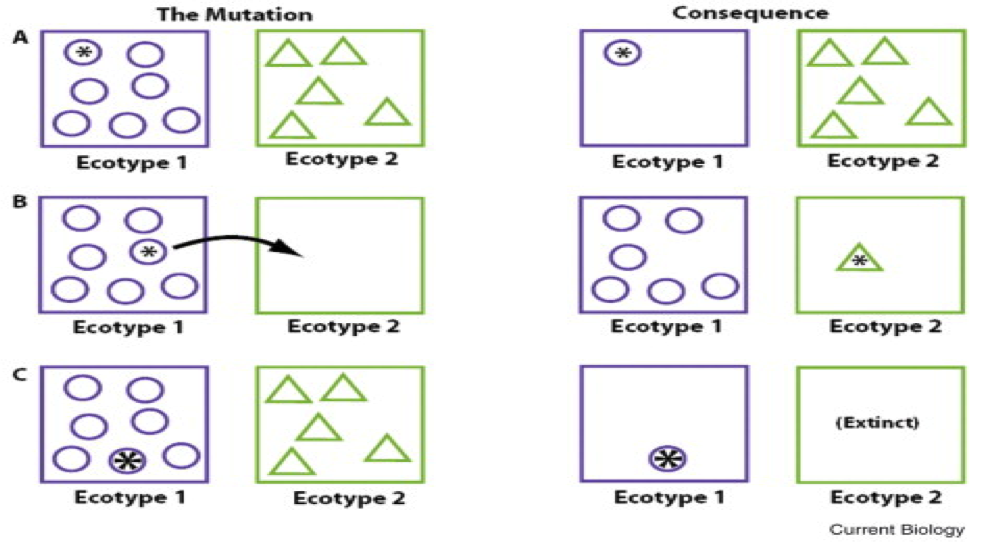
\includegraphics{images/StableEcotypeEvents-CH2}
 \caption[Events predicted by the Stable Ecotype model \protect\cite{cohan2007systematics}.]{Three classes of mutation and recombination events that determine ecotype diversity in bacteria. Circles represent different genotypes, and asterisks adaptive mutations. (A) Periodic selection purges diversity. (B) Ecotype formation creates diversity. (C) Extinction events (reprinted from \protect\cite{cohan2007systematics}).}
\end{figure}

In the Stable Ecotype model ecotypes are created and extinguished at a very low rate, and during its long lifetime an ecotype is recurrently purged of its diversity by periodic selection events~\cite{cohan2007systematics}.
Ecotypes are formed rarely enough so that they can accumulate its own set of unique mutations while diversity is purged, yielding a correspondence between ecotypes and sequence clusters for any gene shared among ecotypes~\cite{cohan2008origins}.
This fact, hinted at earlier, is what allows ES to identify separate ecotypes based on environmental function without knowledge of particular phenotypic mutations.
Diversity quashing events are referred to as periodic selection events, see Figure~\ref{fig:StableEvents}a.
An individual of an ecotype acquires a mutation that improves its fitness within that ecological niche, which results in a diversity purge, due to low recombination rates in bacteria, where other organisms in the ecotype without the adaption become extinct.
Genetic drift is another event that results in diversity purges, however it is normally quite rare.

%Describes relationship of periodic selection events and ecotype formation event
Early during speciation, a new ecotype's niche may rely on proportions of resources used and may be vulnerable to extinction by periodic selection caused by an adaptive mutation within the parental ecotype.
However, a single HGT event may transfer the adaptive mutation across ecotypes, and could thereby prevent extinction of one ecotype by another~\cite{cohan2008origins}.
In this case an ecotype formation event occurs, see Figure~\ref{fig:StableEvents}b.
The ecotype-transcending adaptation allowed an ecotype speciation event to occur. In the figure an individual of an ecotype developed an adaptation that went on to colonize a new niche creating a new ecotype.

Now we have an event to account for anagenesis, or accumulation of changes over time along a single lineage, referred to as periodic selection, and cladogenesis, or irreversible splitting of lineages, referred to as ecotype formation.
To complete the dynamics of the Stable Ecotype model, extinction events are also possible, see Figure~\ref{fig:StableEvents}c.
An ecotype, obviously, can go extinct.
Previous work done in the Cohan lab was done to develop an algorithm based on the Stable Ecotype model, which eventually became known as Ecotype Simulation.


\section{The Algorithm}

\begin{SCfigure}
 \caption[Phylogenetic tree representation of typical Stable Ecotype model case \protect\cite{cohan2008origins}.]{ The Stable Ecotype model, in which ecotype formation is relatively rare, and periodic selection events (represented by asterisks, frequently purge all diversity from within each ecotype. Extinct lineages are dotted, while existing ones are solid. Time progresses from bottom to top. This model predicts a one-to-one correspondence between sequence clusters and ecotypes (reprinted from \protect\cite{cohan2008origins}). }
 \centering
 \label{fig:StableTree}
% 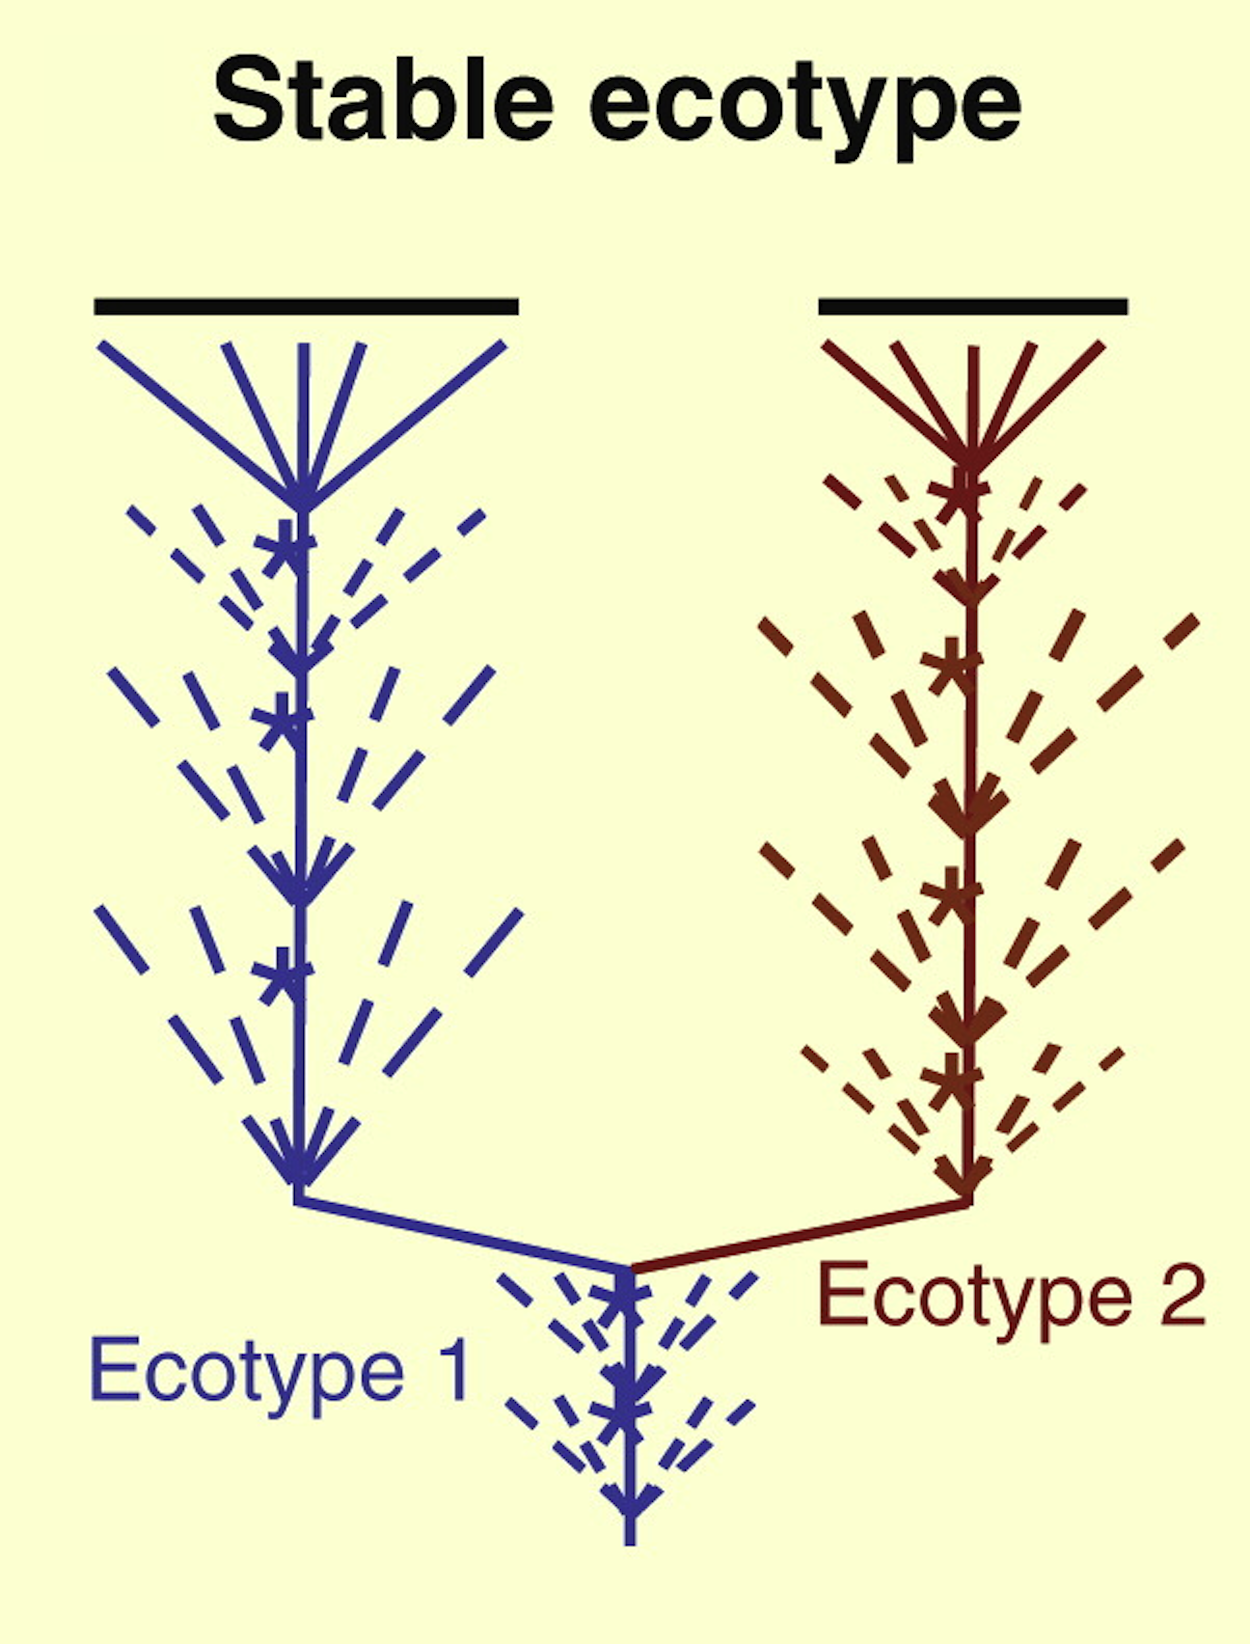
\includegraphics{images/StableTree-CH2}
 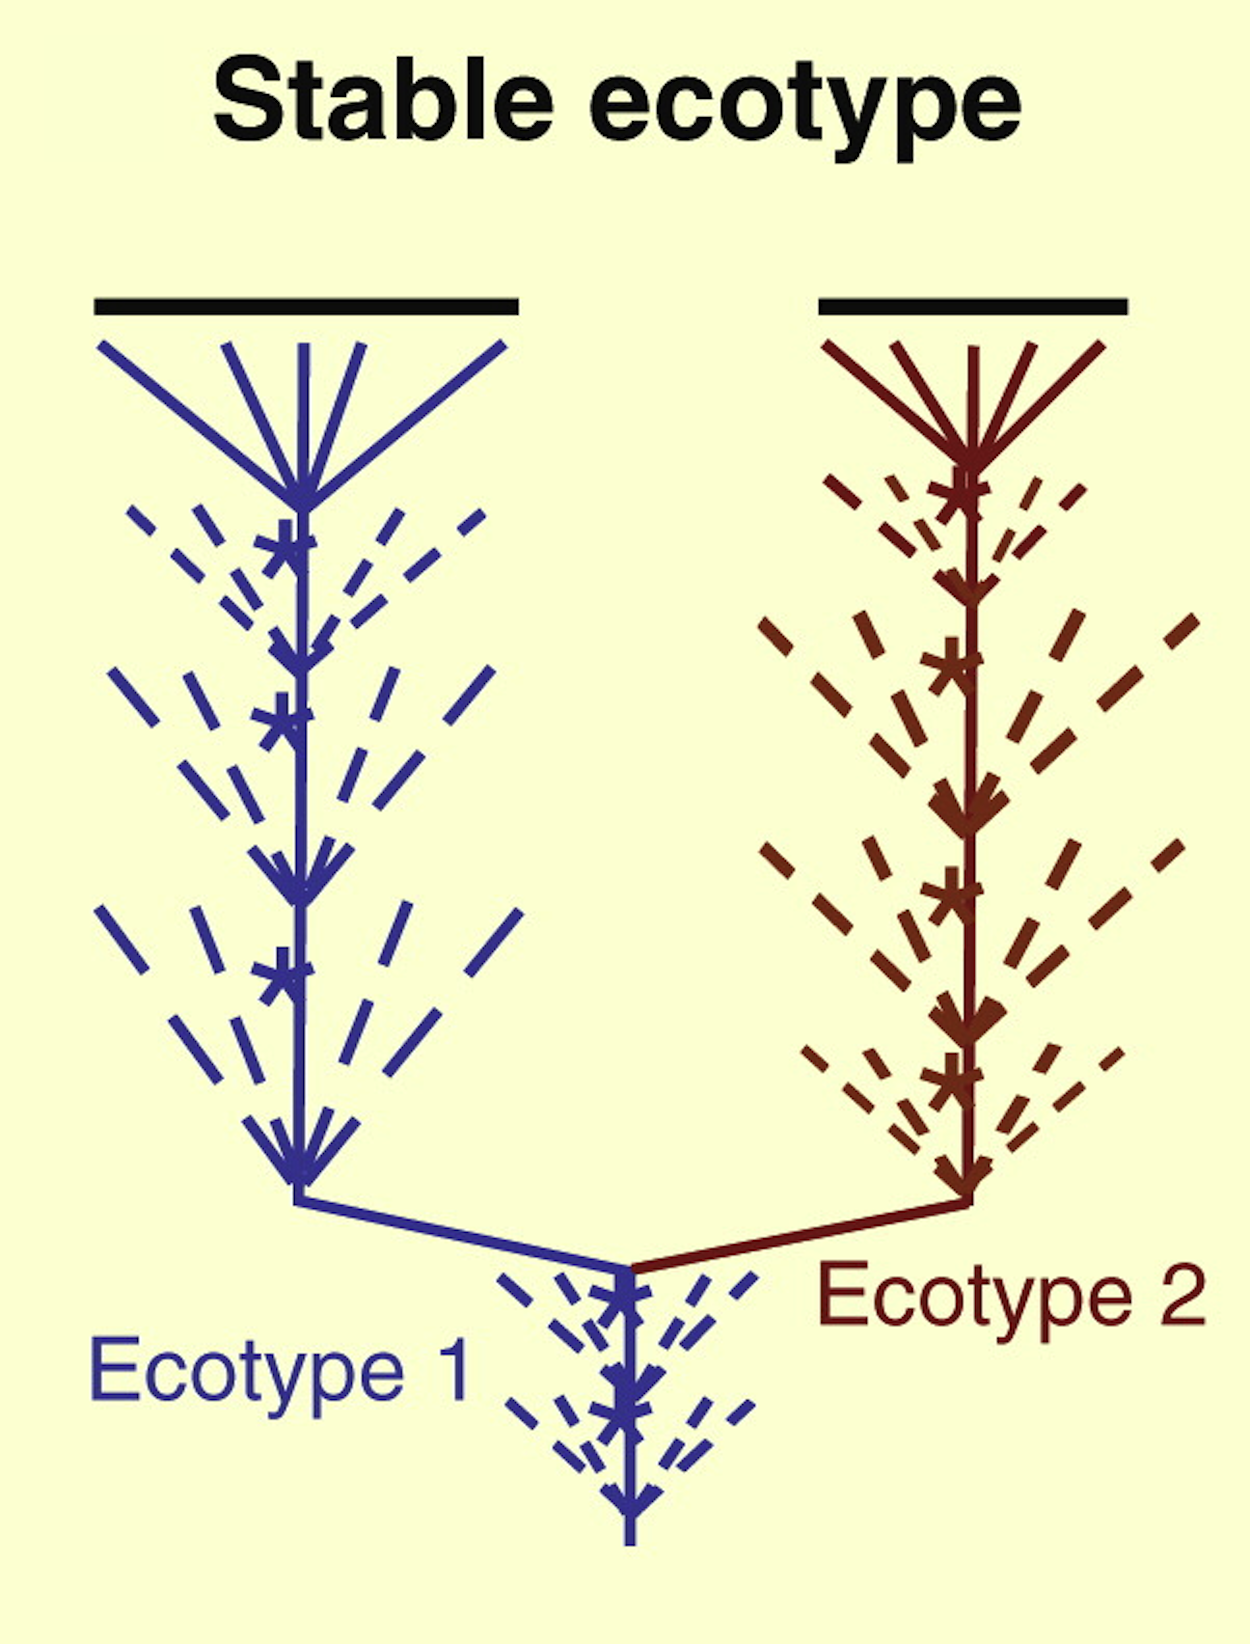
\includegraphics[width=0.5\textwidth]{images/StableTree-CH2}
 %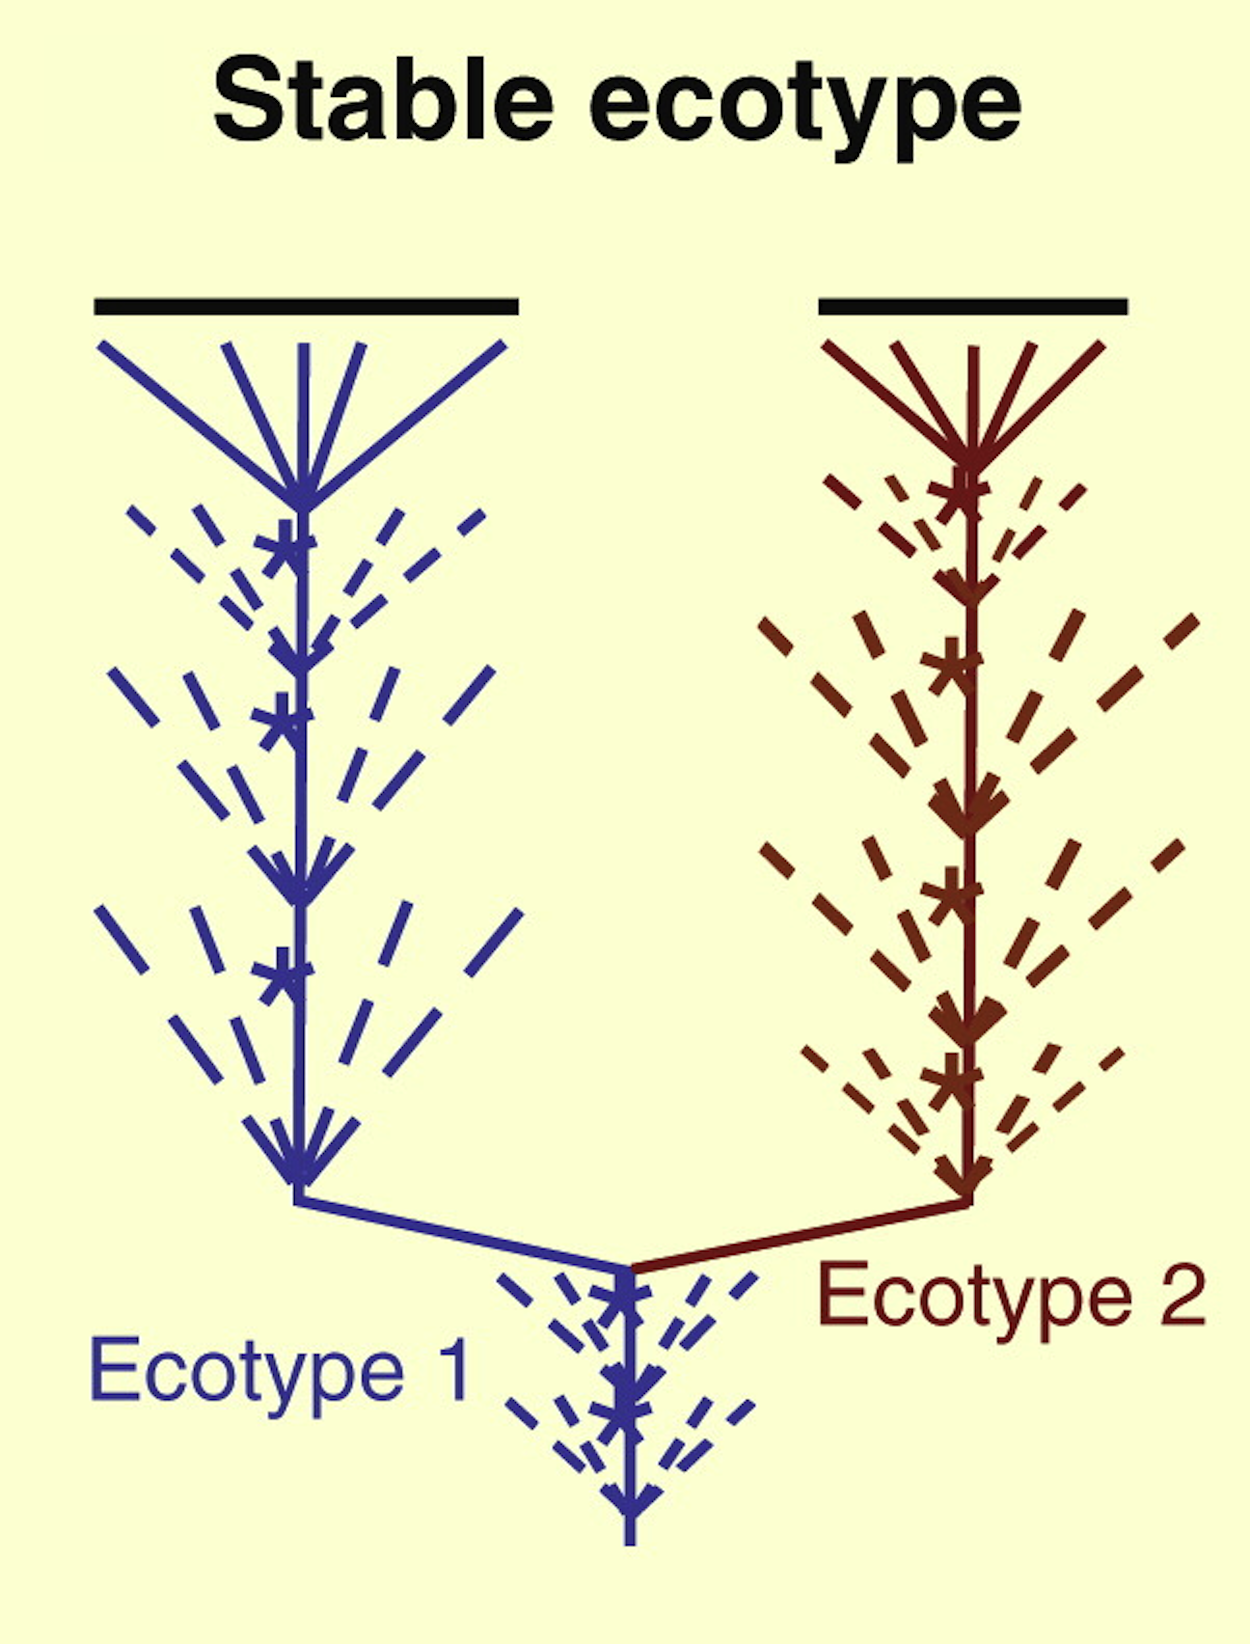
\includegraphics[scale=2.5]{images/StableTree-CH2}
\end{SCfigure}

Utilizing premises established in the Stable Ecotype model we hypothesize a phylogenetic tree similar to the one represented in Figure ~\ref{fig:StableTree}.
Here we can see that ecotype formation is relatively rare, while periodic selection (asterisks) keep the branches of the tree pruned.
At the point of divergence (where the two solid lines separate into ecotype 1 and 2), organisms from the two separate ecotypes are closely related.
However over time and through various purification events adaptive mutations accumulate.
Notice that the two clades are totally free from each other's periodic selection diversity quashing~\cite{cohan2007systematics}.
This is an important feature of separate ecotypes, because we can later observe the differences acquired from separate evolutionary histories.

Theory and empirical evidence hints that these boundaries correlate to ecological niche~\cite{cohan2007systematics, cohan2006sequence, ward2006cyanobacterial, cohan2006toward}.
To identify the system's fundamental elements takes three steps.
First, observe the communities evolutionary history.
Second, simulate evolutionary history as hypotheses of various descriptive parameters, resulting in a most likely parametric characterization of observed history.
Finally, demarcate individuals into ecotypes.

\subsection*{Observing evolutionary history}
Since the clades are evolving independently we can use the molecular clock characteristic of specific ubiquitous genes.
Clearly, the gene we choose to measure between organisms must be present throughout.
For this reason ES typically takes in ribosomal gene 16s, chaperone dnaJ, or gyrase subunit gyrA sequences  as input. Most living organisms have closely related homologues.

From genes we can build a phylogeny that predicts a likely evolutionary history of genes, simply based on sequence distances.
Because, ES only analyzes sequences from non-extinct organisms, the Stable Ecotype model predicts that lineage divergence will be low.
And the bacterial diversity sampled is going through various stages of periodic selection purification, thus the end of the phylogeny (temporally closest to the present) will appear frayed.

\subsection*{Simulating evolutionary history}
Starting from observed sequences as separate clusters, ES simulates common divergence, and cohesion events backwards in time, which reduce the number of groups until there is only one cluster representing the closest ancestor.
From that closest ancestor representation, with known gene mutation rates we can simulate sequence diversity through time and output a virtual gene sequence output.
Now this simulated output can be compared to the observed evolutionary history to check for similarity.
By running many (approximately in the millions) ES develops a max likelihood parametric characterization of the observed phylogeny. 

\subsection*{Demarcating ecotypes}
The parametric characterization helps decide how to separate individuals into clusters.
ES progresses temporally from the root of the phylogeny up analyzing each subtree.
Once there is a certain likelihood that that subtree consists of only one ecotype the demarcation program annotates it as such.


\section{Ecotype Simulation}
%
%   SHOULD WE INCLUDE SAMPLE INPUTS AND OUTPUTS FOR EACH PROGRAM?
%
The current iteration of ES is a GNU General Public Liscenced free (as in freedom, not beer) and open source software written mainly in Fortran90 with a Java graphical user interface (GUI) that runs on most platforms.
As inputs it takes a FASTA format file that consists of aligned DNA gene sequences (usually genes mentioned earlier; concatenated if multiple), and a corresponding phylogeny, either supplied by the user as a Newick format tree or generated by an optional dependency (Phylip ~\cite{felsenstein1989phylip}) on runtime.
The implementation follows our approach discussed in the previous section, namely, observed evolutionary history analysis, simulation, and demarcation.

\subsection*{Binning}
First the input sequences go through pre-processing to remove nucleotide gaps, correct for poly-nucleotide chain reaction (PCR) error.
Next an $O(n^2)$ space divergence matrix is created using a modified Manhattan (or taxicab) distance metric, where at each base pair position if the two sequences being compared differ in nucleotide we increase the distance by one then divide by half the total number of base pairs in the sequence.
The divergence matrix is used to facilitate complete linkage clustering of the sequences, described by the equation $$D(X,Y)= \max_{x\in X, y\in Y} d(x,y)$$ where $d(x,y)$ is the distance between the two elements $x \in X$, and $y \in Y$, and $X$ and $Y$ are two clusters of elements.
The implementation is a naive (i.e., $O(n^3)$) and hoards a lot of space because of the divergence matrix; there is room for improvement here. 

\begin{figure}[h!]
 \centering
 \label{fig:Binning}
 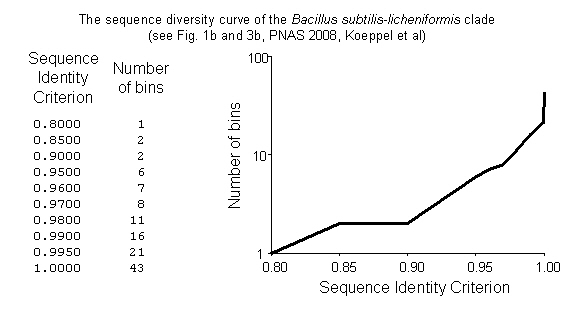
\includegraphics[scale=1.75]{images/Binning-CH2}
 \caption[Sequence identity graph and example output produced by binning \protect\cite{koeppel2008identifying}.]{An example output of information from the initial binning of wild-type sequences (adapted from \protect\cite{koeppel2008identifying}). }
\end{figure}

However, after binning we observe a sequence identity graph as in Figure \ref{fig:Binning}.
The $x$-axis refers to percent identity between sequences and the $y$-axis the number of bins or clusters.
At low sequence identity criterions there are less bins with more sequences in each, and at $1.00$ sequence identity we have unique sequences.
A good way to visualize this sequence identity graph is as a linear representation of a phylogeny.
The slope is shallow during lower sequence identities as in a tree we typically see low levels of cladogenesis.
As you approach the end of a tree there typically is a fraying of the tips, and in the identity graph there is a corresponding steepening of slope, see Figure \ref{fig:SpeciationGraph}. %why isn't this correct?

We can describe the essence of this graph in four parameters: $npop$, sigma ($\sigma$), omega ($\Omega$), and drift (d), which represent the number of ecotypes, rate of periodic selection (PS), rate of ecotype formation (EF), and drift (d), respectively.
By finding close approximations of npop, $\sigma$, $\Omega$, and d we can observe ecotype boundaries within the clade that hypothetically correspond to ecological niche.

\subsection*{Simulations and likelihood evaluation}
The simulation aspect of ES begins with a process of backwards simulation that stochastically (like a roll of a dice) produces a phylogenetic representation of the history of the community.
Think of a node that represents each input sequence (i.e., number of nodes equals number of input sequences) which coalesce (due to PS, EF, or D; indicated by gray circles in Figure \ref{fig:SpeciationGraph}) as ES steps backward in time.
Backwards simulation serves as a scaffold for a forward simulation, which produces corresponding mutational nucleotide substitution throughout the history of the clade.

Initially a set of $v$ contemporary organisms (representing the ones sampled from the environment) are randomly distributed among $n$ ecotypes (in the case of Figure \ref{fig:SpeciationGraph}, $v = 14$, and $n = 3$).
Working backward from the $v$ organisms in the present, the process of EF, PS, and D occur stochastically in time according to their respective predetermined rates ($\Omega$, $\sigma$, and d).
Each event coalesce one or more lineages into  a single ancestral lineage.
The backward phase of the simulation ends when all of the branches have coalesced into a single node, which represents the most recent common ancestor of the sampled organisms.

%EDIT CAPTION
\begin{figure}[h!]
%INCLUDE?
%Note that in the backward-looking view of the coalescence formulation, each PS appears as a coalescence event, in which all lineages after the PS coalesce into the survivor of the PS event. Likewise, each D event appears in this backward-looking view as the coalescence of a pair of lineages within an ecotype (e.g., two contemporary lineages coalesce into lineage D1 to reflect the increased representation of lineage D1 after the random loss by drift of lineage D2). 
%Because $\Omega$ is the net rate of EF events, taking into account extinction, we include in the simulation only those EF events resulting in ecotypes that survive into our contemporary sample.

  \centering
   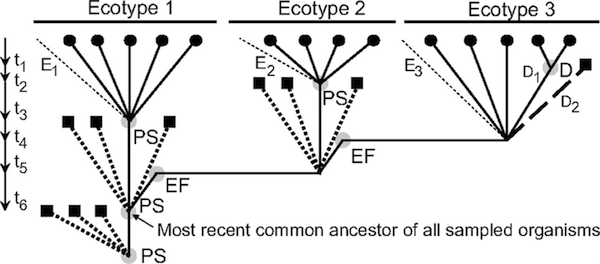
\includegraphics{images/Speciation-CH2}
   \caption[Detailed phylogeny with putative ecotype simulation events \protect\cite{koeppel2008identifying}.]{A phyolgeny representation of the ecotype simulation algorithm. The algorithm simulates the evolutionary history of the organisms sampled from nature under different values for the net rate of ecotype formation (EF), rates of periodic selection (PS), drift (D), and the number of ecotypes in the sample. It only considers existing individuals (black circles) from non-extinct lineages represented by bold lines. Previously extinguished lineages, due to past PS or D events, are represented by dotted lines and squares (reprinted from \protect\cite{koeppel2008identifying}).}
   \label{fig:SpeciationGraph}
\end{figure}

Forward simulation begins when a sequence, the same length of a sample individual, is assigned to the most recent common ancestor.
As time progresses nucleotide substitutions occur stochastically between each pair of nodes (according to the time between the events determining the nodes) in the phylogeny derived from the backward simulation. 
This continues until we reach the contemporary organism nodes, resulting in a matrix of pairwise sequence divergence between $v$ contemporary organisms.

Now ES can conduct the same complete-linkage clustering analysis described in the previous section to illustrate a sequence identity graph, which can be compared to the observed sequence identity graph.
If we place our simulated sequence identity graph line on top of the observed sequence identity graph at each bin level we can see within a pre-determined factor (or wiggle room error) if the simulated line matches the observed line.
Success is determined by whether or not these two lines match within this factor of closeness.
If the simulation and observed graphs are too far apart, ES records the repetition as a failure.
Based on many (i.e., in the hundreds) of runs, each one evaluated for success or failure, we gather information to form a max likelihood estimation of $npop$, $\Omega$, $\sigma$, and d. However, how does one decide on variables?

\subsection*{Bruteforce and Hillclimbing}
Utilizing simulations explained in the previous section ES conducts a search for high likelihoods over a multi-dimensional plane (four parameters).
To search as much of that space as possible we lay a grid of points over that grid of likelihoods where each point is a simulation of many hundred repetitions.
By running those tests we begin to observe a rough sketch of hills and valleys of likely parameters.
The even distribution of points with a lack of insight is referred to as Bruteforce (see Figure \ref{fig:Flow}a).
Bruteforce outputs a range of parameters that should contain some local maximum likelihood.

The range of likely parameters is then passed through an optimization program known as Hillclimbing (see Figure \ref{fig:Flow}b).


\begin{figure}[h!]
 \centering
 \label{fig:Flow}
 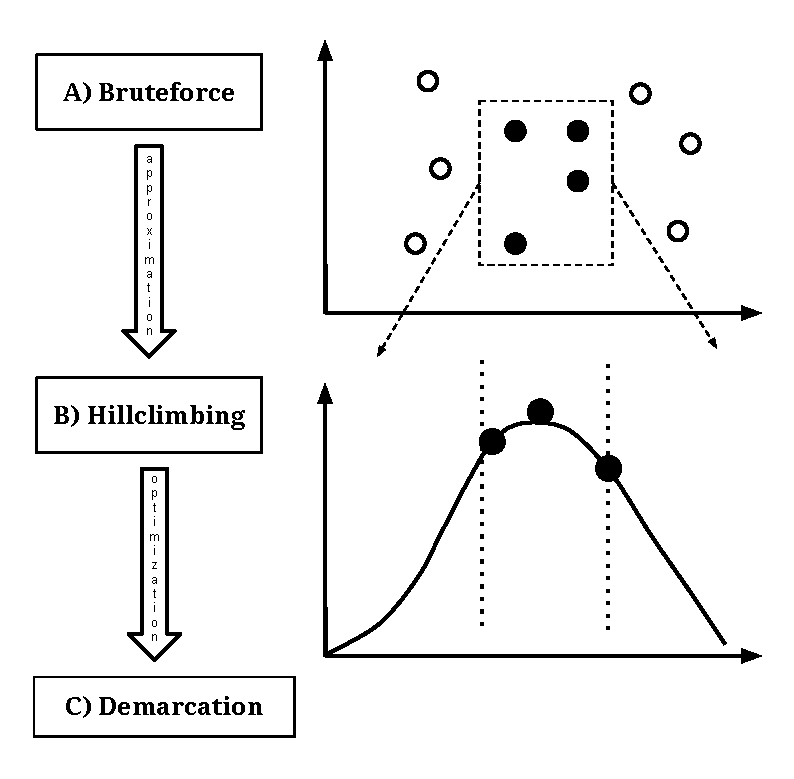
\includegraphics[scale=0.75]{images/ESFlow-CH2.pdf}
 \caption[Ecotype Simulation program flow diagram.]{This is the program call flow of ES. Circles represent simulations, filled are high likelihood successes, while empty are failures. Bruteforce distributes test parameters along the grid, and Hillclimbing figuratively climbs the likelihood hill to find local a maximum (figure created with help from Lingyuan Ke). }
\end{figure}

\subsection*{Demarcation}
With most likely estimations of $npop$, $\sigma$, $\Omega$ we proceed to Demarcation (see Figure \ref{fig:Flow}c).
